% Options for packages loaded elsewhere
% Options for packages loaded elsewhere
\PassOptionsToPackage{unicode}{hyperref}
\PassOptionsToPackage{hyphens}{url}
\PassOptionsToPackage{dvipsnames,svgnames,x11names}{xcolor}
%
\documentclass[
  letterpaper,
  DIV=11,
  numbers=noendperiod]{scrartcl}
\usepackage{xcolor}
\usepackage{amsmath,amssymb}
\setcounter{secnumdepth}{-\maxdimen} % remove section numbering
\usepackage{iftex}
\ifPDFTeX
  \usepackage[T1]{fontenc}
  \usepackage[utf8]{inputenc}
  \usepackage{textcomp} % provide euro and other symbols
\else % if luatex or xetex
  \usepackage{unicode-math} % this also loads fontspec
  \defaultfontfeatures{Scale=MatchLowercase}
  \defaultfontfeatures[\rmfamily]{Ligatures=TeX,Scale=1}
\fi
\usepackage{lmodern}
\ifPDFTeX\else
  % xetex/luatex font selection
\fi
% Use upquote if available, for straight quotes in verbatim environments
\IfFileExists{upquote.sty}{\usepackage{upquote}}{}
\IfFileExists{microtype.sty}{% use microtype if available
  \usepackage[]{microtype}
  \UseMicrotypeSet[protrusion]{basicmath} % disable protrusion for tt fonts
}{}
\makeatletter
\@ifundefined{KOMAClassName}{% if non-KOMA class
  \IfFileExists{parskip.sty}{%
    \usepackage{parskip}
  }{% else
    \setlength{\parindent}{0pt}
    \setlength{\parskip}{6pt plus 2pt minus 1pt}}
}{% if KOMA class
  \KOMAoptions{parskip=half}}
\makeatother
% Make \paragraph and \subparagraph free-standing
\makeatletter
\ifx\paragraph\undefined\else
  \let\oldparagraph\paragraph
  \renewcommand{\paragraph}{
    \@ifstar
      \xxxParagraphStar
      \xxxParagraphNoStar
  }
  \newcommand{\xxxParagraphStar}[1]{\oldparagraph*{#1}\mbox{}}
  \newcommand{\xxxParagraphNoStar}[1]{\oldparagraph{#1}\mbox{}}
\fi
\ifx\subparagraph\undefined\else
  \let\oldsubparagraph\subparagraph
  \renewcommand{\subparagraph}{
    \@ifstar
      \xxxSubParagraphStar
      \xxxSubParagraphNoStar
  }
  \newcommand{\xxxSubParagraphStar}[1]{\oldsubparagraph*{#1}\mbox{}}
  \newcommand{\xxxSubParagraphNoStar}[1]{\oldsubparagraph{#1}\mbox{}}
\fi
\makeatother


\usepackage{longtable,booktabs,array}
\usepackage{calc} % for calculating minipage widths
% Correct order of tables after \paragraph or \subparagraph
\usepackage{etoolbox}
\makeatletter
\patchcmd\longtable{\par}{\if@noskipsec\mbox{}\fi\par}{}{}
\makeatother
% Allow footnotes in longtable head/foot
\IfFileExists{footnotehyper.sty}{\usepackage{footnotehyper}}{\usepackage{footnote}}
\makesavenoteenv{longtable}
\usepackage{graphicx}
\makeatletter
\newsavebox\pandoc@box
\newcommand*\pandocbounded[1]{% scales image to fit in text height/width
  \sbox\pandoc@box{#1}%
  \Gscale@div\@tempa{\textheight}{\dimexpr\ht\pandoc@box+\dp\pandoc@box\relax}%
  \Gscale@div\@tempb{\linewidth}{\wd\pandoc@box}%
  \ifdim\@tempb\p@<\@tempa\p@\let\@tempa\@tempb\fi% select the smaller of both
  \ifdim\@tempa\p@<\p@\scalebox{\@tempa}{\usebox\pandoc@box}%
  \else\usebox{\pandoc@box}%
  \fi%
}
% Set default figure placement to htbp
\def\fps@figure{htbp}
\makeatother


% definitions for citeproc citations
\NewDocumentCommand\citeproctext{}{}
\NewDocumentCommand\citeproc{mm}{%
  \begingroup\def\citeproctext{#2}\cite{#1}\endgroup}
\makeatletter
 % allow citations to break across lines
 \let\@cite@ofmt\@firstofone
 % avoid brackets around text for \cite:
 \def\@biblabel#1{}
 \def\@cite#1#2{{#1\if@tempswa , #2\fi}}
\makeatother
\newlength{\cslhangindent}
\setlength{\cslhangindent}{1.5em}
\newlength{\csllabelwidth}
\setlength{\csllabelwidth}{3em}
\newenvironment{CSLReferences}[2] % #1 hanging-indent, #2 entry-spacing
 {\begin{list}{}{%
  \setlength{\itemindent}{0pt}
  \setlength{\leftmargin}{0pt}
  \setlength{\parsep}{0pt}
  % turn on hanging indent if param 1 is 1
  \ifodd #1
   \setlength{\leftmargin}{\cslhangindent}
   \setlength{\itemindent}{-1\cslhangindent}
  \fi
  % set entry spacing
  \setlength{\itemsep}{#2\baselineskip}}}
 {\end{list}}
\usepackage{calc}
\newcommand{\CSLBlock}[1]{\hfill\break\parbox[t]{\linewidth}{\strut\ignorespaces#1\strut}}
\newcommand{\CSLLeftMargin}[1]{\parbox[t]{\csllabelwidth}{\strut#1\strut}}
\newcommand{\CSLRightInline}[1]{\parbox[t]{\linewidth - \csllabelwidth}{\strut#1\strut}}
\newcommand{\CSLIndent}[1]{\hspace{\cslhangindent}#1}



\setlength{\emergencystretch}{3em} % prevent overfull lines

\providecommand{\tightlist}{%
  \setlength{\itemsep}{0pt}\setlength{\parskip}{0pt}}



 


\KOMAoption{captions}{tableheading}
\makeatletter
\@ifpackageloaded{caption}{}{\usepackage{caption}}
\AtBeginDocument{%
\ifdefined\contentsname
  \renewcommand*\contentsname{Table of contents}
\else
  \newcommand\contentsname{Table of contents}
\fi
\ifdefined\listfigurename
  \renewcommand*\listfigurename{List of Figures}
\else
  \newcommand\listfigurename{List of Figures}
\fi
\ifdefined\listtablename
  \renewcommand*\listtablename{List of Tables}
\else
  \newcommand\listtablename{List of Tables}
\fi
\ifdefined\figurename
  \renewcommand*\figurename{Figure}
\else
  \newcommand\figurename{Figure}
\fi
\ifdefined\tablename
  \renewcommand*\tablename{Table}
\else
  \newcommand\tablename{Table}
\fi
}
\@ifpackageloaded{float}{}{\usepackage{float}}
\floatstyle{ruled}
\@ifundefined{c@chapter}{\newfloat{codelisting}{h}{lop}}{\newfloat{codelisting}{h}{lop}[chapter]}
\floatname{codelisting}{Listing}
\newcommand*\listoflistings{\listof{codelisting}{List of Listings}}
\makeatother
\makeatletter
\makeatother
\makeatletter
\@ifpackageloaded{caption}{}{\usepackage{caption}}
\@ifpackageloaded{subcaption}{}{\usepackage{subcaption}}
\makeatother
\usepackage{bookmark}
\IfFileExists{xurl.sty}{\usepackage{xurl}}{} % add URL line breaks if available
\urlstyle{same}
\hypersetup{
  pdftitle={Exploratory Data Analysis: Wisconsin Diagnostic Breast Cancer (WDBC)},
  pdfauthor={Hoi Hin Kwok, Sameel Syed, Lavanya Gupta \& Yusheng Li},
  colorlinks=true,
  linkcolor={blue},
  filecolor={Maroon},
  citecolor={Blue},
  urlcolor={Blue},
  pdfcreator={LaTeX via pandoc}}


\title{Exploratory Data Analysis: Wisconsin Diagnostic Breast Cancer
(WDBC)}
\author{Hoi Hin Kwok, Sameel Syed, Lavanya Gupta \& Yusheng Li}
\date{}
\begin{document}
\maketitle


\subsubsection{1.1 Introduction}\label{introduction}

This report analyzes the Wisconsin Diagnostic Breast Cancer (WDBC)
dataset to identify key features distinguishing malignant from benign
tumors. The data features were computed from digitized images of fine
needle aspirates (FNA) of breast masses, describing the characteristics
of the cell nuclei present in the image (Wolberg et al. 2003) .

\subsubsection{1.2 Data Acquisition}\label{data-acquisition}

The raw data was retrieved directly from the UCI Machine Learning
Repository to ensure reproducibility. The dataset consists of 569
instances with 30 real-valued input features and one binary target
variable (\texttt{Diagnosis}).

\subsubsection{2. Data Cleaning, Schema Mapping, and Data
Validation}\label{data-cleaning-schema-mapping-and-data-validation}

The raw dataset lacks semantic column headers. To facilitate analysis,
we implemented a schema mapping strategy based on the
\texttt{wdbc.names} metadata. The 30 features represent ten distinct
cell nucleus characteristics (e.g., Radius, Texture) computed in three
statistical forms.

We applied the following suffix mapping transformation: * \textbf{Mean
Value:} Suffix \texttt{1} -\textgreater{} \texttt{\_mean} *
\textbf{Standard Error:} Suffix \texttt{2} -\textgreater{} \texttt{\_se}
* \textbf{Worst (Max) Value:} Suffix \texttt{3} -\textgreater{}
\texttt{\_max}

This step ensures all features are semantically interpretable for the
subsequent EDA.

To ensure the dataset is clean, consistent, and ready for modeling, we
validated the data by implementing the following checks:

\begin{itemize}
\item
  Correct Data File Format The cleaned dataset was exported as a
  standard CSV (breast\_cancer\_cleaned.csv) with UTF-8 encoding. It
  successfully loaded in pandas without errors, confirming proper file
  format and readability.
\item
  Correct Column Names All 30 feature columns follow the expected naming
  convention (\_mean, \_se, \_max). The Diagnosis column contains only
  ``Benign'' and ``Malignant'' values, and the total number of columns
  is 31, as expected.
\item
  No Empty Observations All rows contain complete observations. There
  are no fully empty rows, and no partial missing values were detected.
\item
  Missingness Within Expected Threshold A threshold of 5\% missingness
  per column was applied. No columns exceeded this limit, ensuring all
  features are sufficiently complete for reliable modeling.
\end{itemize}

By combining schema mapping with these validation checks, the dataset is
fully consistent, correctly formatted, and reproducible, providing a
robust foundation for downstream modeling and analysis.

\subsubsection{Outlier Analysis \& Scaling
Strategy}\label{outlier-analysis-scaling-strategy}

Due to the massive disparity in magnitude between features (e.g.,
\texttt{Area} \textgreater{} 2000 vs.~\texttt{Smoothness} \textless{}
0.2), a \textbf{Symmetric Log (Symlog) scale} was applied to the
visualizations. This effectively mitigates the compressing effect of the
\texttt{Area} feature, allowing the distribution and spread of
smaller-scale variables to be clearly observed without losing the
information from larger values.

Post-scaling inspection reveals numerous outliers (points beyond
whiskers), particularly in Malignant samples (Orange). *
\textbf{Significance:} These are \textbf{not data errors}. In the
context of breast cancer, extreme values in features like \texttt{Area},
\texttt{Concavity}, and \texttt{Perimeter} are characteristic of
malignant tumor growth. * \textbf{Conclusion:} These points represent
high-priority \textbf{biological signals} essential for classification.

\textbf{Preprocessing Recommendation} * \textbf{Action:} \textbf{Do not
drop} these outliers, as removing them would discard critical diagnostic
information. * \textbf{Strategy:} To handle the skewness and scale
differences during modeling: 1. Apply \textbf{Log Transformation}
(\texttt{np.log1p}) to right-skewed features (Area, Perimeter) to
normalize distributions. 2. Apply \textbf{Standard Scaling}
(\texttt{StandardScaler}) to all features to ensure the model treats all
dimensions with equal weight.

\begin{enumerate}
\def\labelenumi{\arabic{enumi}.}
\setcounter{enumi}{8}
\tightlist
\item
  Target/response variable follows expected distribution
\end{enumerate}

\begin{itemize}
\tightlist
\item
  We validate that the target variable \texttt{Diagnosis} is not
  severely imbalanced. If one class is much rarer than the other, this
  can hurt model performance and may require special handling (for
  example, resampling or adjusting evaluation metrics).
\end{itemize}

\begin{enumerate}
\def\labelenumi{\arabic{enumi}.}
\tightlist
\item
  No anomalous correlations between target and features
\end{enumerate}

\begin{itemize}
\tightlist
\item
  We check how strongly each feature is associated with
  \texttt{Diagnosis}. Extremely high predictive power for a single
  feature can indicate data leakage or unexpected dependencies that
  should be investigated.
\end{itemize}

\begin{enumerate}
\def\labelenumi{\arabic{enumi}.}
\tightlist
\item
  No anomalous correlations between features
\end{enumerate}

\begin{itemize}
\tightlist
\item
  We examine pairwise correlations between features. If many feature
  pairs are highly correlated, this suggests redundancy or
  multicollinearity, which may require feature selection or
  dimensionality reduction.
\end{itemize}

The \texttt{FeatureFeatureCorrelation} check fails the condition we set.
In our data there are many feature pairs with very high correlation, for
example \texttt{radius\_mean}, \texttt{perimeter\_mean} and
\texttt{area\_mean}, as well as their corresponding \texttt{\_max} and
\texttt{\_se} versions. This pattern is expected for this dataset
because these variables all describe related geometric properties of the
tumor, so strong correlations are not a data quality error but a sign of
redundancy and multicollinearity.

\subsubsection{3. Data Profiling: Structure and
Statistics}\label{data-profiling-structure-and-statistics}

\textbf{Purpose:} * \textbf{\texttt{df.info()}:} Used to verify data
integrity by checking for null values and ensuring all feature columns
are of \texttt{float64} type. * \textbf{\texttt{df.describe()}:} Used to
examine the central tendency and spread of numeric features. This
highlights differences in \textbf{magnitude} (scales) across variables.

\textbf{Observation:} The dataset is complete (no missing values).
However, \texttt{describe()} reveals massive scale disparities (e.g.,
\texttt{area\_mean} ranges up to 2500, while \texttt{smoothness\_mean}
is \textless{} 0.1), confirming the necessity for \textbf{Feature
Scaling} (Standardization) before modeling.

\subsubsection{4. Correlation Analysis: Pearson
vs.~Spearman}\label{correlation-analysis-pearson-vs.-spearman}

\textbf{Method:} * \textbf{Pearson Correlation:} Measures linear
relationships. * \textbf{Spearman Correlation:} Measures monotonic rank
relationships (non-linear). Comparing both helps identify if
relationships are strictly linear or just trending in the same
direction.

\textbf{Purpose:} To detect \textbf{Multicollinearity}---redundant
features that increase model complexity without adding information.

\textbf{Results:} Both metrics show near-perfect correlation (\(>0.95\))
between \texttt{Radius}, \texttt{Perimeter}, and \texttt{Area}. This
confirms these features are geometrically redundant. We should retain
only one (e.g., Radius) and drop the others to improve model stability.

\begin{figure}

\centering{

\pandocbounded{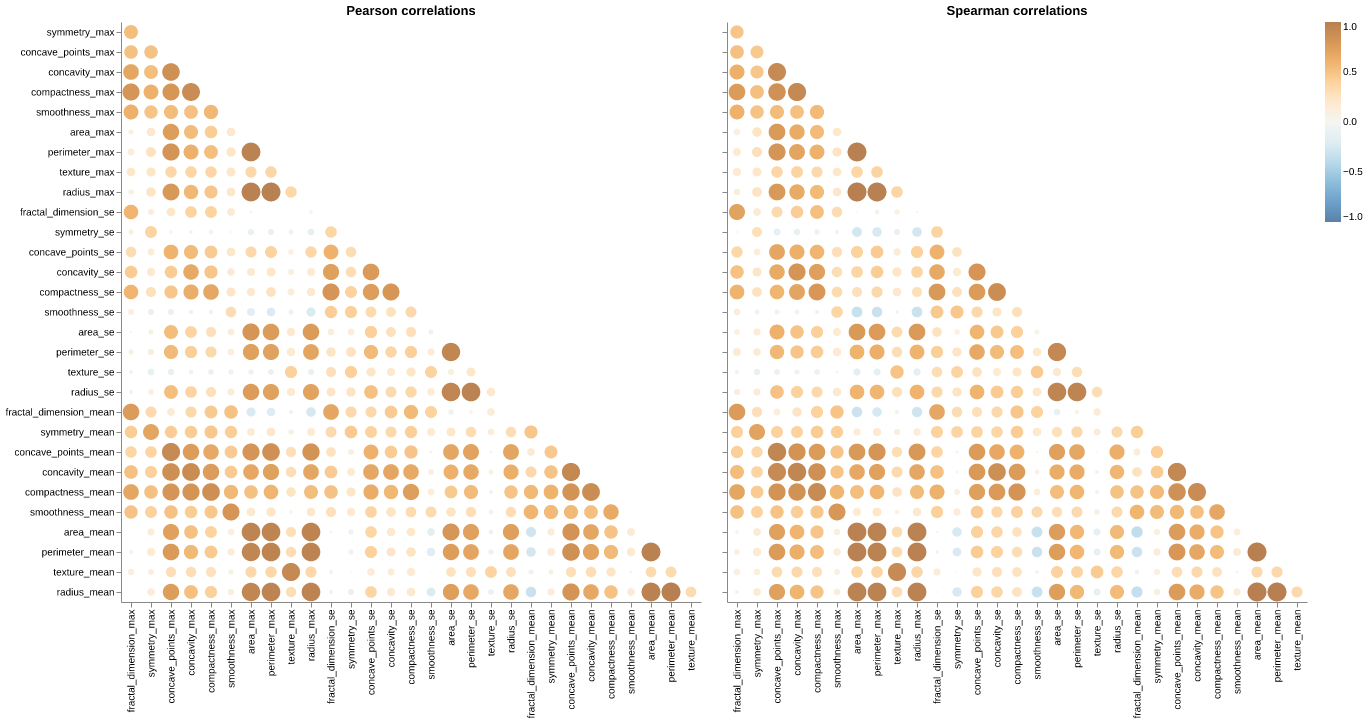
\includegraphics[keepaspectratio]{../results/images/corr_chart.png}}

}

\caption{\label{fig-corr_chart}Multicollinearity}

\end{figure}%

\subsubsection{5. Pairwise Separability
Analysis}\label{pairwise-separability-analysis}

\textbf{Purpose:} To visualize 2D decision boundaries. We look for
feature combinations where the \textbf{Benign (Blue)} and
\textbf{Malignant (Orange)} clusters are clearly distinct with minimal
overlap.

\textbf{Results:} * \textbf{High Separability:} Features related to size
(\texttt{radius\_mean}) and shape complexity (\texttt{concavity\_mean})
separate the classes well. * \textbf{Non-linear patterns:} The curved
relationship between \texttt{area} and \texttt{radius} is clearly
visible, reinforcing the geometric redundancy found in the correlation
analysis.

\subsubsection{6. Distribution Analysis}\label{distribution-analysis}

\textbf{Purpose:} To inspect the univariate ``shape'' of the data. We
look for \textbf{Skewness} (asymmetry) and \textbf{Outliers} that could
bias linear models.

\textbf{Results:} * \textbf{Skewness:} Features like \texttt{area\_se}
and \texttt{concavity\_mean} are heavily \textbf{right-skewed} (long
tail to the right). This indicates that \textbf{Log Transformation} is
required to normalize these distributions. * \textbf{Overlap:}
``Texture'' and ``Smoothness'' show high overlap between classes,
suggesting they are less informative on their own compared to ``Size''
features.

\subsubsection{EDA Findings}\label{eda-findings}

\begin{itemize}
\tightlist
\item
  \textbf{Class Separation:}

  \begin{itemize}
  \tightlist
  \item
    \textbf{High Separability:} Features related to \textbf{size}
    (\texttt{radius}, \texttt{perimeter}, \texttt{area}) and
    \textbf{concavity} (\texttt{concave\_points}, \texttt{concavity})
    show clear distinction between Benign and Malignant classes
    (Malignant samples generally have higher values).
  \item
    \textbf{Low Separability:} Texture, Smoothness, and Fractal
    Dimension show significant overlap, indicating they are weaker
    individual predictors.
  \end{itemize}
\item
  \textbf{Distributions:}

  \begin{itemize}
  \tightlist
  \item
    \textbf{Skewness:} ``Area'' and ``Concavity'' features (both
    \texttt{\_mean} and \texttt{\_se}) are heavily
    \textbf{right-skewed}.
  \item
    \textbf{Outliers:} Visible in the upper tails of \texttt{area\_max}
    and \texttt{perimeter\_se}.
  \end{itemize}
\item
  \textbf{Correlations (Multicollinearity):}

  \begin{itemize}
  \tightlist
  \item
    \textbf{Severe Multicollinearity:} \texttt{radius},
    \texttt{perimeter}, and \texttt{area} are perfectly correlated
    (\(R \approx 1\)). This is expected geometrically but redundant for
    models.
  \item
    \texttt{concavity}, \texttt{concave\_points}, and
    \texttt{compactness} also exhibit very high positive correlation.
  \end{itemize}
\end{itemize}

\subsubsection{Preprocessing
Recommendations}\label{preprocessing-recommendations}

Based on the above, the following pipeline is suggesued:

\begin{enumerate}
\def\labelenumi{\arabic{enumi}.}
\tightlist
\item
  \textbf{Feature Selection / Drop:}

  \begin{itemize}
  \tightlist
  \item
    Remove redundant features to reduce multicollinearity. \textbf{Keep
    \texttt{radius}} (or \texttt{perimeter}), but \textbf{drop
    \texttt{area}} and \texttt{perimeter} as they duplicate information.
  \end{itemize}
\item
  \textbf{Transformation:}

  \begin{itemize}
  \tightlist
  \item
    Apply \textbf{Log Transformation} to skewed features (e.g.,
    \texttt{area}, \texttt{concavity}) to normalize distributions.
  \end{itemize}
\item
  \textbf{Scaling:}

  \begin{itemize}
  \tightlist
  \item
    Features vary vastly in scale (e.g., \texttt{area} \textgreater{}
    1000 vs.~\texttt{smoothness} \textless{} 0.2). Use
    \textbf{\texttt{StandardScaler}} to standardize all features to unit
    variance.
  \end{itemize}
\item
  \textbf{Imputation:}

  \begin{itemize}
  \tightlist
  \item
    None needed (Data is clean).
  \end{itemize}
\end{enumerate}

\subsubsection{Onto Creating a Classification
Model}\label{onto-creating-a-classification-model}

\begin{figure}

\centering{

\pandocbounded{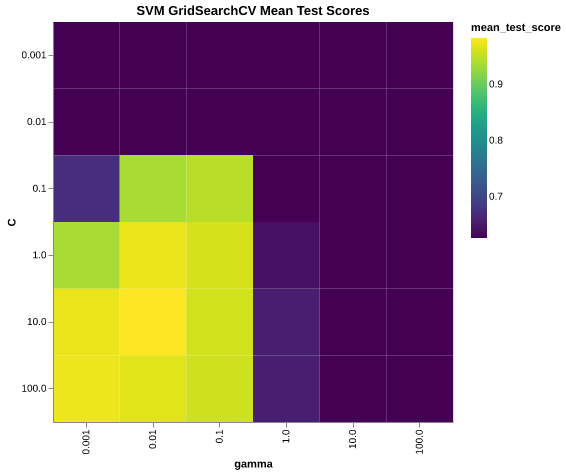
\includegraphics[keepaspectratio]{../results/images/svm_heatmap.png}}

}

\caption{\label{fig-svm_heatmap}Heatmap for SVM GridSearchCV Mean Test
Score}

\end{figure}%

\begin{figure}

\centering{

\pandocbounded{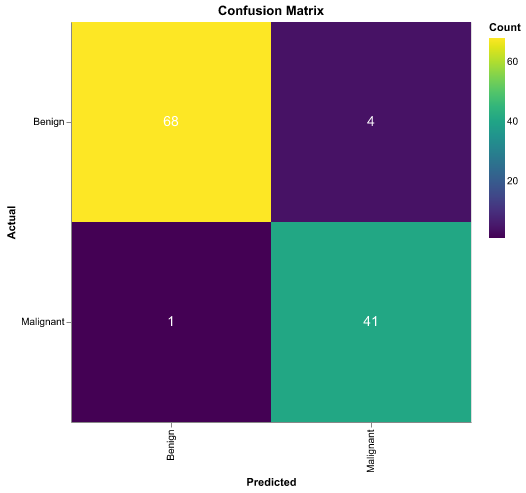
\includegraphics[keepaspectratio]{../results/images/con_mat_heatmap.png}}

}

\caption{\label{fig-con_mat_heatmap}Heatmap for Confusion Matrix}

\end{figure}%

\subsubsection{Discussion:}\label{discussion}

Our model demonstrated strong performance, achieving high accuracy on
the test set derived from the UCI Machine Learning Repository (Frank
2010) and correctly classifying nearly all cases. This result was
generally expected given the strong feature patterns observed during
Exploratory Data Analysis (EDA), which suggested a clear separation
between benign and malignant tumours.

However, the main concern is the occurrence of a single false negative,
where a malignant tumour was incorrectly predicted as benign. Although
rare, such an error carries significant clinical risk. Accurate
classification is critical for determining appropriate treatment
pathways (Board 2025), and missed diagnoses can severely impact patient
outcomes given the prevalence and nature of the disease (Society 2007).
This highlights that the model, while statistically strong, requires
further refinement before it is reliable enough for real-world medical
deployment.

These results suggest that future work should explore methods aimed at
reducing false negatives, such as adjusting class weights, employing
cost-sensitive training, or validating on external datasets to assess
robustness.

\subsubsection*{References}\label{references}
\addcontentsline{toc}{subsubsection}{References}

\phantomsection\label{refs}
\begin{CSLReferences}{1}{0}
\bibitem[\citeproctext]{ref-board2025breast}
Board, PDQ Adult Treatment Editorial. 2025. {``Breast Cancer Treatment
(PDQ{\textregistered}).''} \emph{PDQ Cancer Information Summaries
{[}Internet{]}}.

\bibitem[\citeproctext]{ref-frank2010uci}
Frank, Andrew. 2010. {``UCI Machine Learning Repository.''}
\emph{Http://Archive. Ics. Uci. Edu/Ml}.

\bibitem[\citeproctext]{ref-american2007breast}
Society, American Cancer. 2007. \emph{Breast Cancer Facts \& Figures}.
American Cancer Society.

\bibitem[\citeproctext]{ref-wolberg2003elevated}
Wolberg, Alisa S, Dougald M Monroe, Harold R Roberts, and Maureane
Hoffman. 2003. {``Elevated Prothrombin Results in Clots with an Altered
Fiber Structure: A Possible Mechanism of the Increased Thrombotic
Risk.''} \emph{Blood, The Journal of the American Society of Hematology}
101 (8): 3008--13.

\end{CSLReferences}




\end{document}
